\section{Auswertung}
Die zu beginn des Versuchs durchgeführte Nullmessung ergibt die in Abb.\ref{Leermessung} dargestellte Energieverteilung. Sie zeigt deutlich den bei $^{137}$Cs auftretenden Peak um $662 \, \si{\kilo\electronvolt}$ sowie die davor liegende
Compton-Kante. Es wurden $11059$ Ereignisse in $60.42 \, \si{\second}$, oder $183 \,  \pm \, 3\, \frac{\text{counts}}{\si{\second}}$ gemessen.
Die in den Spektren gezeigten Fehlerbalken stammen von den, durch die Poisson-Verteilung gegebenen, $\sqrt{n}$ Fehler.
\begin{figure}[H]
  \centering
  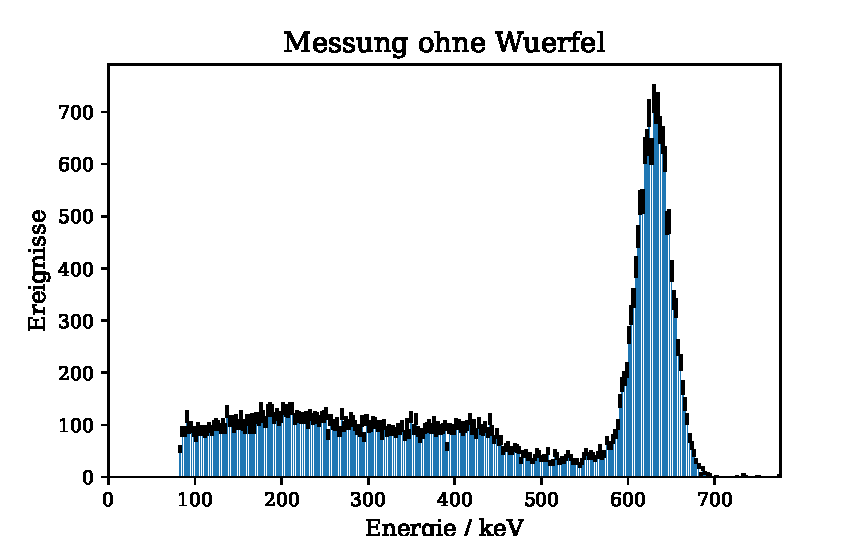
\includegraphics{plots/leer.pdf}
  \caption{Schematische Darstellung des Versuchsaufbaus.\cite{anleitung}}
  \label{Leermessung}
\end{figure}
\subsection{Leerer Würfel}
Die Untersuchungen des leeren Würfels ergeben die in Abb.\ref{Wurfelleer} gezeigten Spektren. Der Intensitätsvektor
für die verschiedenen Projektionen der ersten Messung sind in (7) zu finden, die der zweiten in (8).
Aufgrund des homogenen Aufbaus des Würfels,
werden für nicht vermessene Projektionsrichtungen die Werte von äquivalenten Projektionen eingesetzt.
Vermessen wurden die Projektionsrichtungen 1, 3, 13, 14, 15

\begin{equation}
	\vec{I_1}=
	\begin{pmatrix}
		\num{180.1 \pm 2.4} \\
		\num{180.1 \pm 2.4} \\
		\num{180.1\pm 2.4} \\
		\num{178.8\pm 2.4} \\
		\num{178.8\pm 2.4} \\
		\num{178.8\pm 2.4} \\
		\num{176.6\pm 2.4} \\
		\num{177.0\pm 2.4} \\
		\num{175.9\pm 2.4} \\
    \num{176.6\pm 2.4} \\
    \num{177.0\pm 2.4} \\
    \num{175.9\pm 2.4} \\
	\end{pmatrix}
    \sfrac{\text{counts}}{\text{s}}
	\label{eq:vecleer1}
\end{equation}
\begin{equation}
	\vec{I_2}=
	\begin{pmatrix}
		\num{171.7 \pm 2.4} \\
		\num{171.7 \pm 2.4} \\
		\num{171.7\pm 2.4} \\
		\num{173.3\pm 2.4} \\
		\num{173.3\pm 2.4} \\
		\num{173.3\pm 2.4} \\
		\num{165.2\pm 2.4} \\
		\num{161.8\pm 2.4} \\
		\num{174.1\pm 2.4} \\
    \num{165.2\pm 2.4} \\
    \num{162.8\pm 2.4} \\
    \num{174.1\pm 2.4} \\
	\end{pmatrix}
    \sfrac{\text{counts}}{\text{s}}
	\label{eq:vecleer2}
\end{equation}
\subsection{Untersuchung der Würfel 2 und 3}
